\newpage

\chapter{提案手法}

  本章では,プロシージャルモデリングにおける操作パラメータを削減したシステムの提案を行う.

\section{システム}
\subsection{システム概要}
図\ref{fig:systemFlow},\ref{fig:systemUI}に提案システムのフロー図およびシステムUI の概略図を示す.また,図\ref{fig:systemAno}に実装したシステムを示す.
図\ref{fig:systemAno}について,


まず操作1では,UI 上の数字のボタンによって番号に対応する提案モデルを3つ選択する.
次に操作2で三角形のUIで赤色のポインタを操作することにより,選択された3つのモデルの補間を行う.この時,ポインタの位置が三角形の頂点に近づくほど,その点に対応するモデルに近づく.
そして操作3は ADJ ボタンを押すことで,各パラメータを個別に調節できるサイドバーを表示することが出来る.それによって従来のプロシージャルモデリングと同じく個別の調整が可能となる.
そして, NEXT ボタンを押すことで提案モデルを変更していく.


以上の操作を何度も繰り返すことで,自身の好きなモデルを生成していく.そして最後に END ボタンによって操作を終了する.また,フロー図上では簡略化のため選択と補間を一方通行に記載しているが,実装上では選択中の数字のボタンを再度押すことで選択を外すことが出来,その後別の数字ボタンを押して補間対象のモデルに別の提案モデルを設定することが出来る.
\clearpage

また図\ref{fig:systemUI}に示すように,前述した操作に加え HIDE ボタンを実装する.これは,操作モデル以外を一時的に非表示,再表示する機能を持つ.補間操作によってモデルのサイズが大きくなり,提案モデルや補間対象のモデルと重なる場合がある.その場合に操作の邪魔になるため,提案するシステム操作に対して新たに組み込んだ.

\begin{figure}[h]
    \centering
  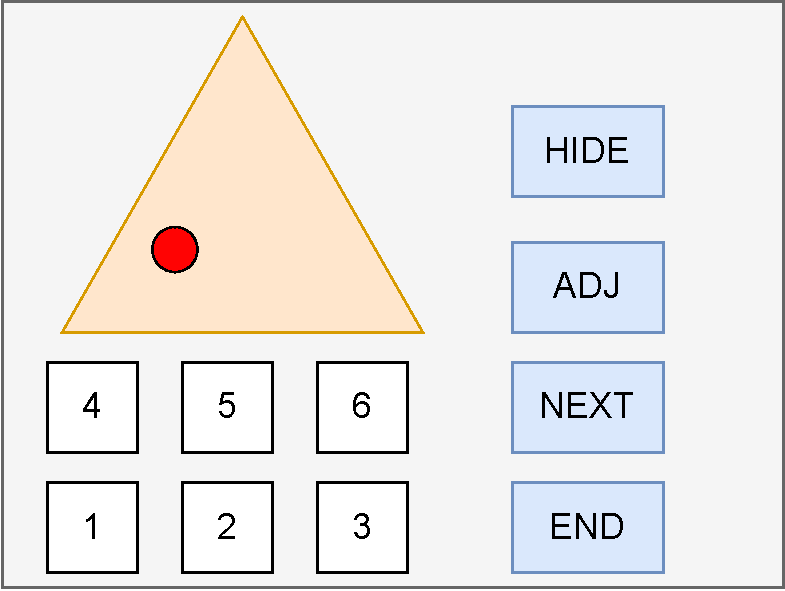
\includegraphics[width=0.55\textwidth]{./imgs/systemUI.pdf}
  \caption{システム UI の概略図}\label{fig:systemUI}
\end{figure}

\begin{figure}[h]
    \centering
  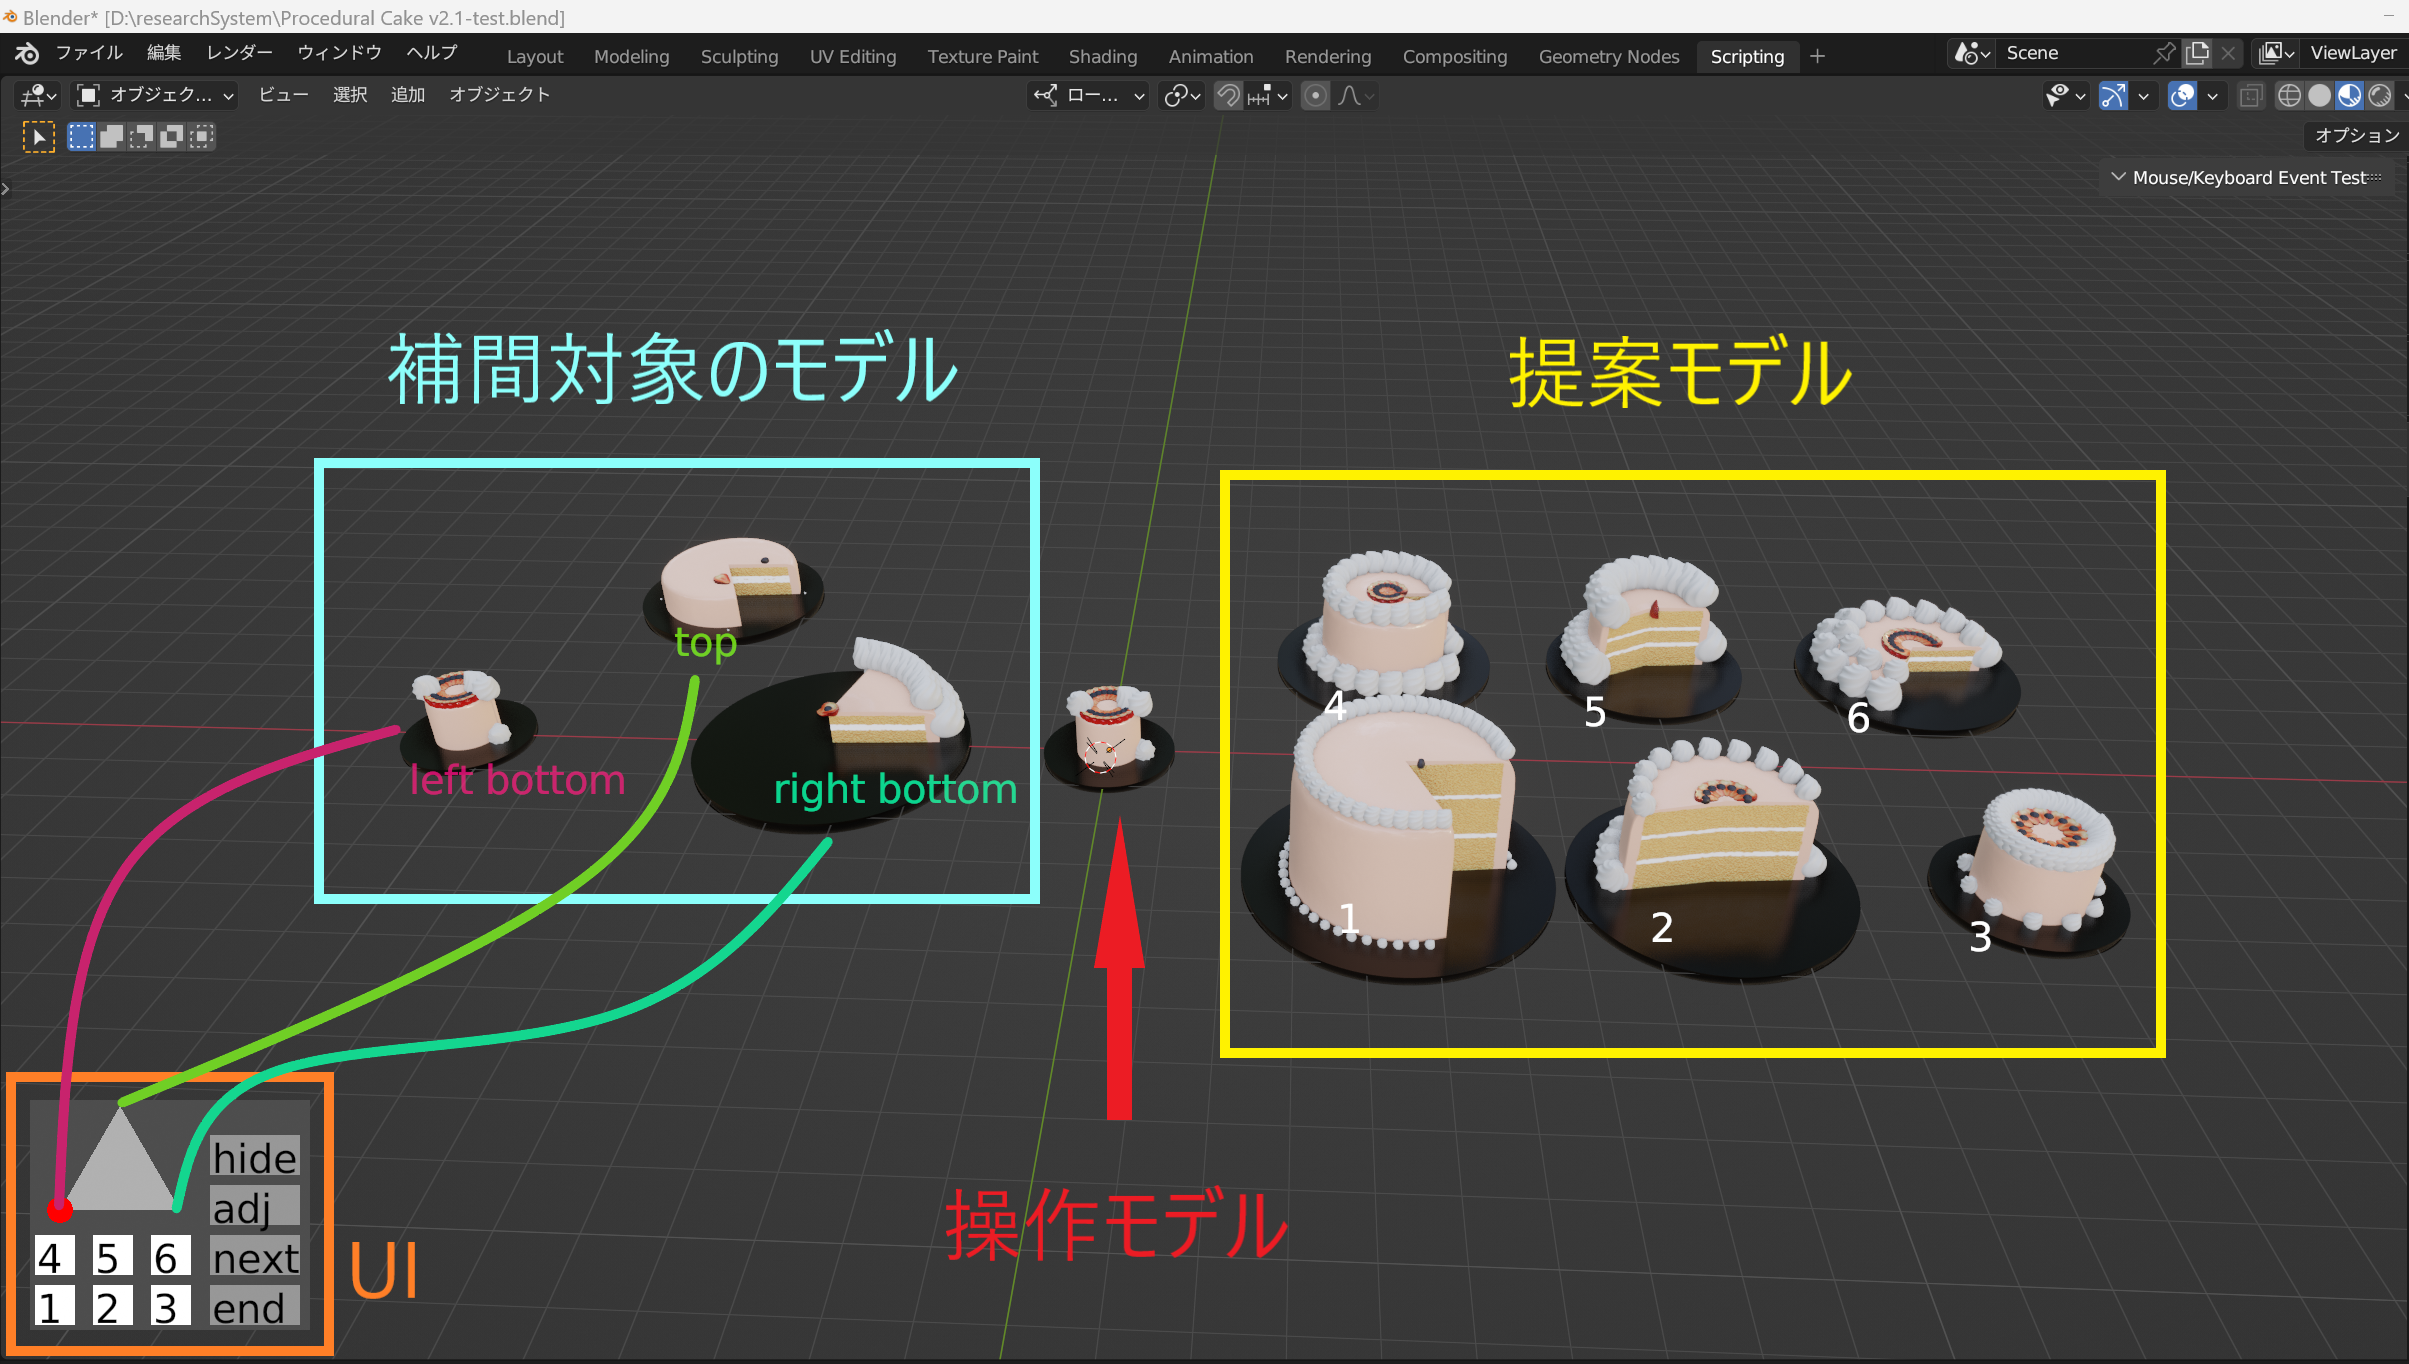
\includegraphics[width=1.0\textwidth]{./imgs/system_ano.png}
  \caption{実装したシステム}\label{fig:systemAno}
\end{figure}

\clearpage
\begin{figure}[h]
    \centering
  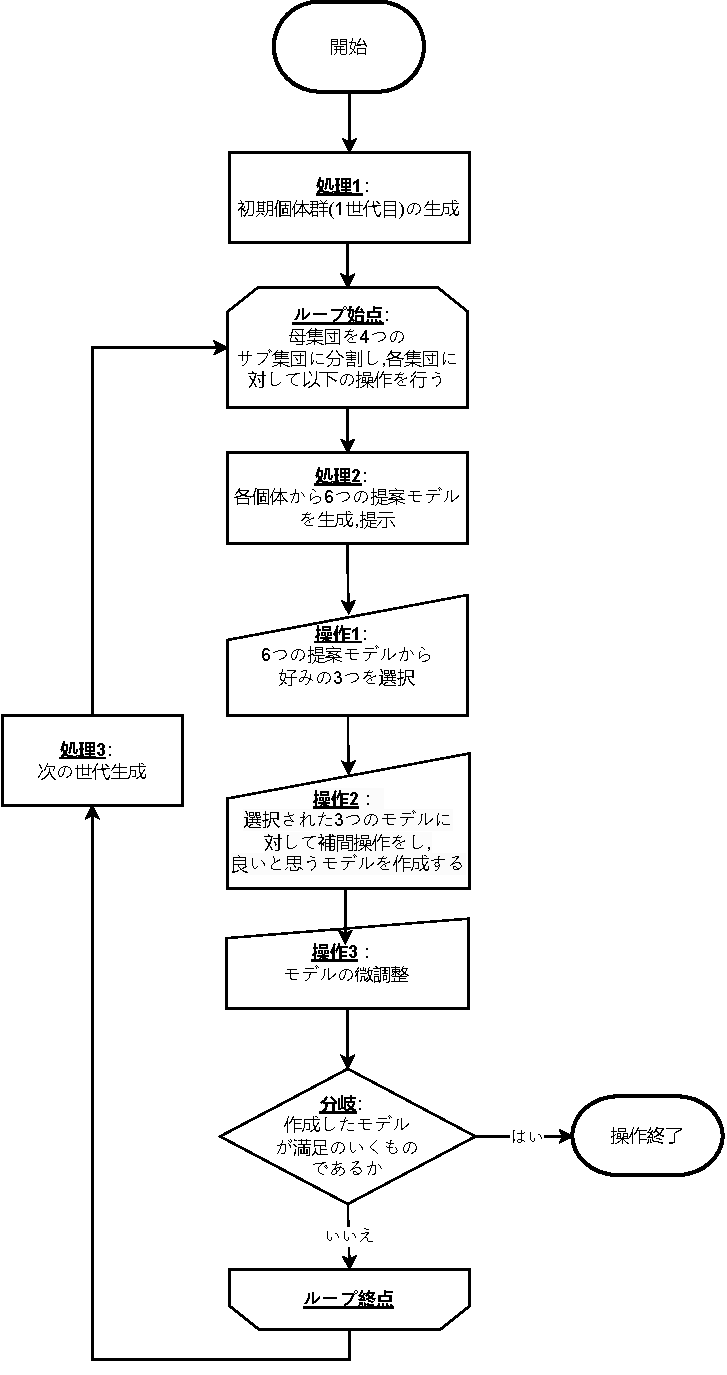
\includegraphics[width=0.7\textwidth]{./imgs/systemFlow.pdf}
  \caption{システムフロー図}\label{fig:systemFlow}
\end{figure}
\clearpage


\subsection{個体表現}
まず,プロシージャルモデリングには様々な入力データが存在する.

\begin{itemize}
      \item 整数値
      \item 実数値
      \item あらかじめ制作された複数のアセット(テクスチャなど)
      \item ストローク
\end{itemize}

提案システムでは,複数の個体を用いたパラメータ補間を行う.そのため,整数値は離散値ではあるため内部的に実数値として処理を行った.式\ref{set:Z},\ref{set:R}が処理を行った前後の集合である.
パラメータ$a$が$[m,n]$の整数値であるとき,$[m,n+1)$の実数値上における同じ値への変換を行い.入力パラメータへの変換は少数以下切り捨てによって行う.

\begin{equation}\label{set:Z}
 \{a | m \leq a \leq n , a\in\mathbb{Z}\}
\end{equation}
\begin{equation}\label{set:R}
 \{a | m \leq a < n + 1 , a\in\mathbb{R}\}
\end{equation}

また,アセットを設定するような入力データについて,補間を行う際にアセットの順序性について検討する必要がある.アセットについても有限個であるため,前述した整数値と同様の処理が内部的に行われ,各整数とアセットとを対応させる.そのため補間が行われるときに常にある順番でアセットが変わることになる.この順序性の検討は本研究の範囲外であるため,今回の実験には含めていない.
さらにストロークによって枝の形状やオブジェクトの配置を指定するようなプロシージャルモデリングの場合,
ストロークに対しては,有限個の頂点情報を結ぶことによって表現されているため,順列コーディングと組み合わせることで表現を行うことはできる.しかし,その表現を補間する手法やそれをシステムUI内で再現することは非常に難解なため,本研究では扱わない.


従って,本研究の遺伝子は全て実数値コーディングとして扱う.また遺伝子長については,実装されたプロシージャルモデリングによって設定されたパラメータによって決定されるため様々であり,本研究では汎用性のあるシステム設計を行うことを考えているため,長さは使用するモデルのパラメータ数に応じた可変長である.

\clearpage
\subsection{システム操作と GA 操作の関係}
提案システムは従来の GA 操作と類似点を持たせるように設計する.これにより1ステップにおける GA 操作を疑似的に増やし,収束速度を速める試みをする.

\subsubsection{選択操作}
複数の選択肢からいくつかを選択するという操作は名前の通りであり,従来の IGA でも同じ操作によって親個体の選択が行われる.ただし,従来のものではより多くの選択肢から選択するが,提案システムでは補間操作を行うことで,選択されたモデル以外のモデルについても閲覧,決定を行う事が出来る.
つまり補間操作を加えた探索範囲は補間対象である3つの個体が存在する平面空間上という制約はあるが,ユーザのドラッグ操作により連続的に行える.
従来の IGA の提案では1ステップでの探索範囲は有限個の提案モデル群のみであり,離散的にしか行えない.
そのため,本システムでは提案モデル数を従来よりも減らしても良いと考える.また,ドラッグ操作の手間はあるものの,選択肢の数を減らすことで一度の意思決定のストレスを減らす事が出来る.

\subsubsection{補間操作}
補間操作はユーザのドラッグ操作によってモデルを連続的に閲覧することが可能であり,
探索された平面空間上においてユーザ評価がより高いモデルを決定する事が出来る.
これは,限定的ではあるが交叉操作に類似している.
図\ref{fig:UNDX}に3つの親個体($\bm{x}1,\bm{x}2,\bm{x}3$)を用いて交叉を行う UNDX の個体生成分布図を示す.この分布は遺伝子数と同じ次元数を持つ多変量正規分布として広がる. UNDX ではこの分布に従って子個体が生成される.ただし, UNDX では正規分布として直線上に子個体が生成されるという点から,変数間の依存性が高いものに強力な一方で広い探索範囲をカバーできない欠点がある.一方で,提案する補間操作では,3つの個体が存在する平面空間という制約上で探索し選択されるという点で類似している.また探索空間を限定する反面,その平面上を隙間なく探索できるためユーザ感性における適応度が最大化した個体を発見する可能性が高いという点では,従来の IGA よりも優位な個体を選別出来ていると考えられる.

\begin{figure}[h]
	\begin{center}
		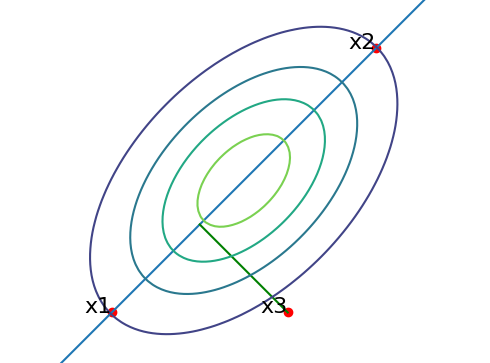
\includegraphics[scale=0.7]{./imgs/UNDX.png}
		\caption[UNDX による個体生成分布図]{ UNDX による個体生成分布図\label{fig:UNDX}}
	\end{center}
\end{figure}


\newpage


次に,4つ以上のより高次元での補間操作ではない理由を説明する.4つ以上の補間操作のほうが,高次元の空間を探索できるというメリットがある一方で,操作難度が高くなるというデメリットがある.平面UIにおける3つの個体の補間操作について,(\ref{eq:rex1})式で与える.
\begin{equation}\label{eq:rex1}
    \bm{x}^c = a*(\bm{x}_\mathrm{top} - \bm{x}_\mathrm{left\ bottom}) + b*(\bm{x}_\mathrm{right\ bottom} - \bm{x}_\mathrm{left\ bottom})
\end{equation}


ここで,$\mathbf{x}^c$は補間個体,$\mathbf{x}_\mathrm{top},\mathbf{x}_\mathrm{left\ bottom},\mathbf{x}_\mathrm{right\ bottom}$は補間操作UIにおける選択されたモデルであり,図\ref{fig:systemAno}においてUIの三角形の頂点と曲線で結ばれたモデルとが対応している.このとき重み変数$a,b$は(\ref{eq:weight})式が成り立つものとする.
\begin{equation}\label{eq:weight}
    \bm{p}_\mathrm{cursor} - \bm{p}_\mathrm{left\ bottom}  = a*(\bm{p}_\mathrm{top} - \bm{p}_\mathrm{left\ bottom}) + b*(\bm{p}_\mathrm{right\ bottom} - \bm{p}_\mathrm{left\ bottom})
\end{equation}
ここで, $\bm{p}_\mathrm{cursor}, \bm{p}_\mathrm{left\ bottom}, \bm{p}_\mathrm{top}, \bm{p}_\mathrm{right\ bottom}$はそれぞれ画面座標の原点から操作ポインタ,三角形UIの左下頂点,上頂点,右下頂点へのベクトルである.すなわち,左下頂点からポインタへのベクトルを上頂点,右下頂点方向の二つのベクトルで表すときの重みが$a,b$である.このようにすることで,$a,b$は行列計算で簡単に解く事が出来る.このように表すことで,操作ポインタと各頂点との距離が、補間対象の各モデルとの距離に対応するため,直感的な補間操作を行う事が出来る.しかし,これが4個以上での補間を二次元である平面 UI 上で実装しようとすると不都合が生じる.異なる四点を結ぶ三角錐状の三次元空間を二次元空間に射影しようとすると次元削減分の情報の損失が起こるため歪みが生じる.それを歪みなくかつドラッグで補間を表現するには,三角錐の断面を並行投影すればいいが,内部を全て探索できるようにするためには断面方向を回転させるといった別の操作が必要になり,操作難度が高くなる.


%\newpage

ここで,図\ref{fig:metahuman_cc2}に MetaHuman のブレンド操作について示す.図\ref{fig:metahuman_cc2}では現在作成しているキャラに加えて,4つのモデルをブレンド対象に使用している.しかし,計5つのモデルに対して補間操作を行っているわけではなく,実際には中心のモデルと,左の円環状に配置された4つのモデルのうち隣り合う二つの計3つのモデルの補間である.現在の対象は図左側のキャラのうち水色でハイライトした3人である.
このブレンド操作では,白のカーソルに近い位置3つのキャラのブレンドが行われる.
そのためカーソルが黄色の円内のどこに位置するかによって補間対象となるモデルが変わってしまう.現在セットされているのは4つのモデルのため,赤の線で4等分した領域ごとに補間対象のモデルが変わる.
現在カーソルが黄色の円内左下にいることから,ブレンド対象のキャラも中心のキャラから見て,左と下のキャラが対象になる.
このように既存のドラッグ操作による補間システムでも3種類が限界であるという事例から分かる通り,
平面のUIで4つ以上の直感的な補間操作を実現することは難しいため,今回は3つの補間操作を採用する.

\begin{figure}[h]
	\begin{center}
		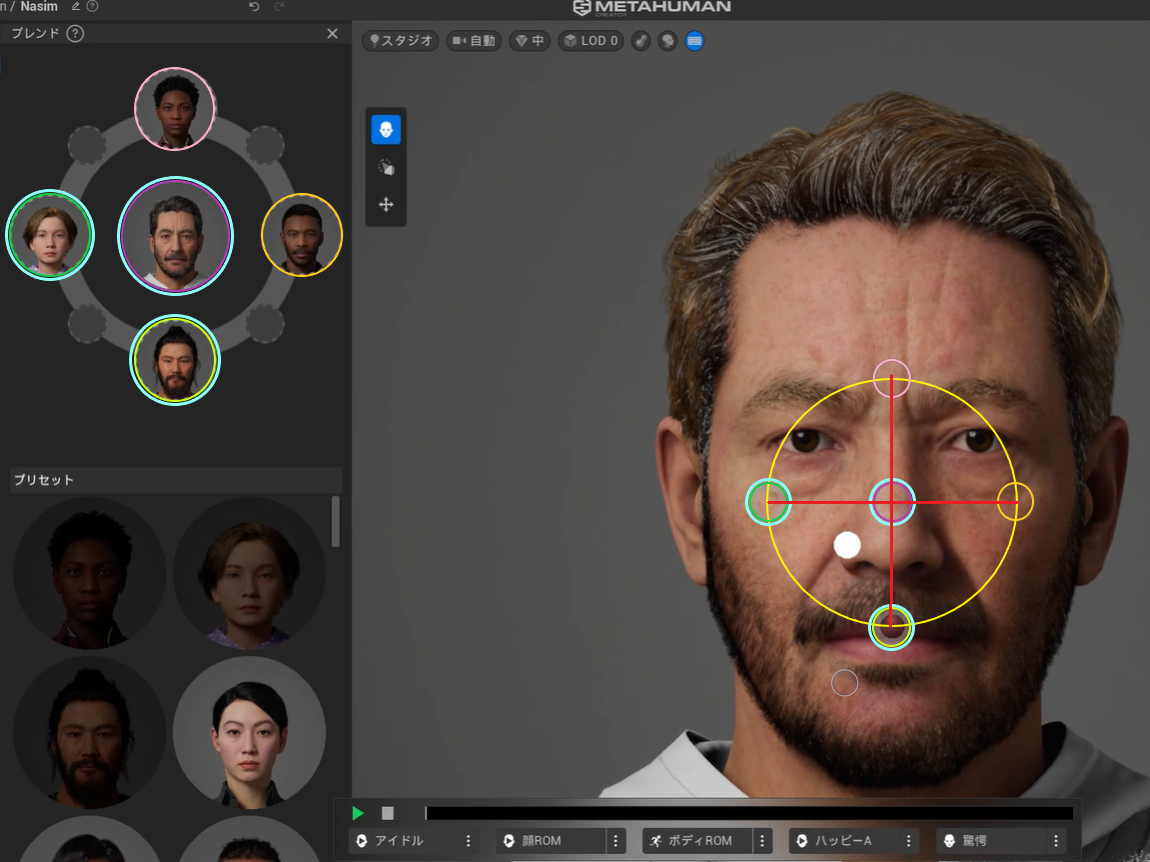
\includegraphics[scale=0.4]{./imgs/metahuman2.PNG}
		\caption{MetaHuman のブレンド操作\label{fig:metahuman_cc2}}
	\end{center}
\end{figure}

\clearpage
\section{IGA による次世代生成}

\subsection{選択}
選択操作は,エリート選択,トーナメント選択の両方によって行う.
エリート選択は補間によって決定されたモデルに対して,次の世代に何も変更を加えずに追加する.
トーナメント選択は選択された個体を親個体として,次の手順である交叉に全て使う.

\subsection{交叉}
交叉については多親交叉 REX を用いる.遺伝子数$n$に任意定数$k$を加えた$n+k$個の親を用いた交叉方法で,親個体群$\bm{x}^1,\bm{x}^2,...,\bm{x}^n+k$の重心を$\bm{x}^\mathrm{g}$としたとき,子個体$\bm{x}^c$は次の式で与えられる.
\begin{equation}\label{eq:rex1}
    \bm{x}^c = \bm{x}^\mathrm{g} + \sum_{i=1}^{n+k} \xi^i (\bm{x}^i - \bm{x}^\mathrm{g}) ,  \xi^i\sim\phi(0,\sigma^2_\xi)
\end{equation}
\begin{equation}\label{eq:rex2}
    \sigma^2_\xi = \frac{1}{n + k}
\end{equation}

この時,$\phi(0,\sigma^2_\xi)$は平均0,分散$\sigma^2_\xi$の確率分布であり,制限として(\ref{eq:rex2})式を満たすことが実数値 GA における設計指針において良い\cite{小林重信2009実数値}とされている.本提案では従来の手法に倣い,確率分布として一様分布を用いる.

\subsection{突然変異}
突然変異率1\%で遺伝子の値が別の値に置き換わるようにする.この値は通常の遺伝的アルゴリズムよりも大きく設定してある.理由として,多親交叉 REX\cite{小林重信2009実数値}での想定として,親個体数が遺伝子長よりも大きくするべきであると記述がある.しかし,本提案手法では親個体数が少ないために収束率が高くなってしまう.そこで突然変異率を上げることで多様性の維持をしつつも,収束は行えるような値に設定した.また,突然変異率が2\%を超えると個体群の分散が1世代で0.9倍程度しか収束しないことを事前に検証しており,世代数が増えてしまうのを防ぐために1\%とした.


また突然変異が起こった際に,変化する値については以下の$(\kappa,\mu)=(0.5,0)$のフォンミーゼス分布\cite{vonMisesDist}を正規化したものに従うものとする.(\ref{eq:von1}),(\ref{eq:von2}),(\ref{eq:von3})式に累積分布関数,確率密度関数,j次の第一種変形ベッセル関数について示す.$\mu$は角度方向のパラメータであり, $[0\mathrm{rad},2\pi \mathrm{rad}]$の間で確率密度における
ピークの方向を示す. $\kappa$は濃度パラメータで,大きいほどピークが高くなる.この時に方向を示す実数値$\theta$がとる確率は$F(\theta)$で表される.図\ref{fig:vonMises50000}に50000サンプルの度数分布表を示す.図\ref{fig:vonMises50000}から見て分かる通り,V字型の確率分布になっている.この確率分布を利用する.提案手法では補間を行う関係上,補間幅が広い方が多くの領域を探索出来ることになるため,補間幅が広くなるような値である定義域の端に近い値に変異してほしいと考えた.従って,一様分布ではなくV字型の分布を持つものを採用する.V字型の分布の中でフォンミーゼス分布を利用する理由として,本システムの実装に用いた Python で容易に実装出来るからである.

\begin{equation}\label{eq:von1}
F(\theta) = \frac{1}{2\pi I_{0}(\kappa)} \left[\theta I_{0}(\kappa) + 2 \sum_{j=0}^{\infty} \frac{I_{j}(\kappa) \sin(j(\theta - \mu))}{j}\right]
\end{equation}
\begin{equation}\label{eq:von2}
f(\theta) = \frac{\exp\{\kappa \cos(\theta - \mu)\}}{2\pi I_{0}(\kappa)}
\end{equation}
\begin{equation}\label{eq:von3}
I_{j}(\kappa) = \left(\frac{\kappa}{2}\right)^{j} \sum_{i=0}^{\infty} \frac{\left(\frac{\kappa^{2}}{4}\right)^{i}}{i!\Gamma(j+i+1)}
\end{equation}

\begin{figure}[h]
	\begin{center}
		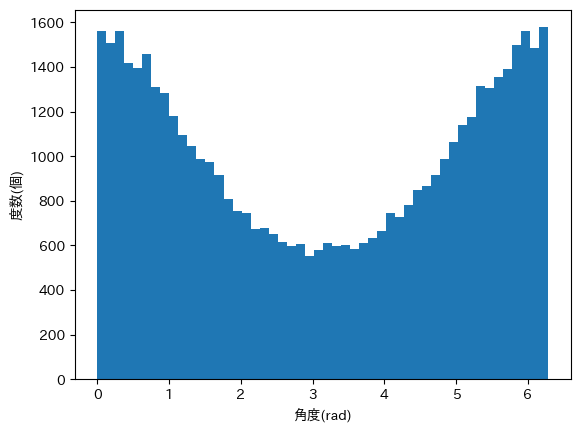
\includegraphics[scale=0.55]{./imgs/vonMisesDis50000.png}
		\caption{フォンミーゼス分布のヒストグラム(sample size = 50000)\label{fig:vonMises50000})}
	\end{center}
\end{figure}
\newpage

\subsection{サブ集団}
IGA における一世代における個体数は24個体に設定し,サブ集団は6個体ずつに4つのサブ集団に分ける.この個体数に関しては,単純なGAであれば20から40個体で十分であるという研究報告\cite{grefenstette1986optimization}があり, IGA の時間的制約のためなるべく小さくしたいという理由からである.またサブ集団の個数設定について,補間を行う個体が3つであるのでその倍数にしたかったという点と,モデリングの際に対象となるモデル以外をあまり多く配置してしまうと,画面を圧迫するために少なくしたかったという点からである.
このようにサブ集団に分けて並列的に行われる手法を島モデル型分散遺伝的アルゴリズム\cite{tanese1989distributed}という.
ただし,本研究では, IGA における一度に提示する提案モデル数の削減が主目的である.
島モデル型では,選択や交叉など各サブ集団ごとに行われるが,
本システムに用いる交叉手法である多親交叉REXは親の数が多く求められるので親個体を分けて交叉はしない.


ここで$k$世代目の$m$番目のサブ集団における補間個体を${\bm{x}^k_m}_\mathrm{elite}$とするとき,表\ref{tb:nextSub}のように$k+1$世代生成を行う.また,図\ref{fig:subFlow}にネットワーク図を示す.

\begin{table}[h]
	\centering
	\caption{$k+1$世代目の個体群\label{tb:nextSub}}
	\scalebox{1.0}{
		\begin{tabular}{|c|c|c|} \hline
                サブ集団番号&エリート個体&交叉生成される個体数\\ \hline\hline
                1&${\bm{x}^k_1}_\mathrm{elite}$&5\\ \hline
                2&${\bm{x}^k_2}_\mathrm{elite}$&5\\ \hline
                3&${\bm{x}^k_3}_\mathrm{elite}$&5\\ \hline
                4&${\bm{x}^k_1}_\mathrm{elite}, {\bm{x}^k_2}_\mathrm{elite}, {\bm{x}^k_3}_\mathrm{elite}, {\bm{x}^k_4}_\mathrm{elite}$&2\\ \hline
		\end{tabular}
	}
\end{table}

\begin{figure}[h]
	\begin{center}
		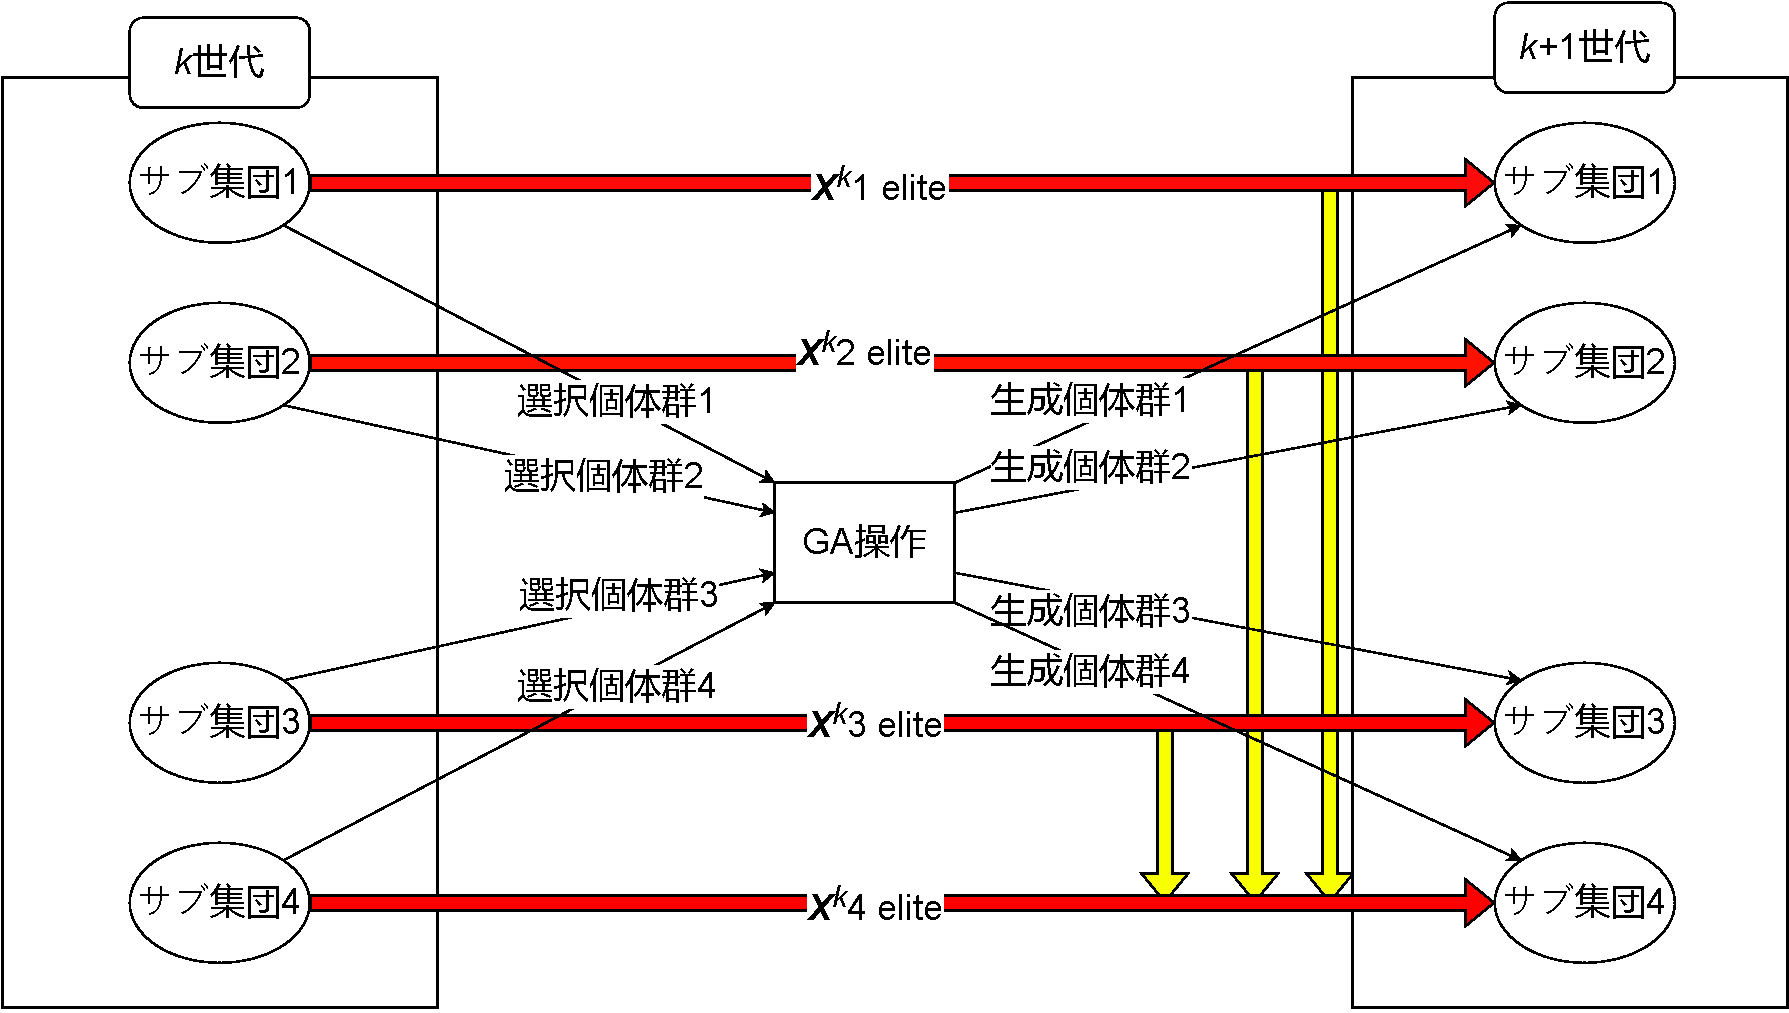
\includegraphics[scale=0.4]{./imgs/subFlow.pdf}
		\caption{次世代生成のネットワーク図\label{fig:subFlow}}
	\end{center}
\end{figure}
つまり,サブ集団1,2,3については1世代前の同サブ集団からエリート個体を引き継ぎ,サブ集団4については1世代前のエリート個体すべてを引き継ぎ,各サブ集団の個体数が6個体になるように個体生成された子個体で埋めた.

このとき24個体中,交叉生成をした子個体は17個体であり,交叉率は71\%である.
1ステップ前に制作したモデルを一新し,前世代のエリート個体を再び提案モデルとして登場させることで,過去の考えを組みつつも新しい発想が生み出されていくことを期待する.加えて,エリート個体をすべて引き継ぐサブ集団4を用意することでより洗練されたモデルが生み出されることを望む.

\newpage

\section{微調整操作}
この操作はプロシージャルモデリングのパラメータを直接操作するという,従来の方法であり,操作パラメータ数の削減という本研究の目的を逸脱している.しかし,提案モデルにユーザが欲しいと思う特徴がない時や,あと少し手を加えたいといったことについて,本システムは補間操作およびIGAによるモデル提案という性質上,そのような細かいモデリングを行うことは難しい.そのため基本操作上ではパラメータ操作のUIは隠しつつも,必要であれば表示して操作が出来るようにすることで,大まかな補間操作に加えて細かいパラメータ調整を適宜行えるようにした.


ただし,この操作は補間モデルだけでなく,選択モデルに対しても行う.なぜなら,補間モデルに対してパラメータ操作した差分を選択モデルに対しても操作をすることで,補間としての体裁を保つことが出来る.また,個別で調整するということはそのパラメータがユーザにとって重要度が高いと言える.そのため,親個体にその要素を引き継ぐ必要がある.以上の2点からパラメータ調整した差分は選択モデルに対しても適用する.

\section{システムインターフェース}
本節ではシステムインターフェースについて,各操作を3段階ずつ示すことで,操作に対する動作を説明する.
図\ref{fig:systemOverViewInit}はシステムの初期状態である.左下に UI ,
中心のモデルが操作されるモデル,右6つのモデルが提案されるモデル,左3つは補間対象であるモデルが表示される.


まず図\ref{fig:systemOverViewSelect}に選択操作を示す.選択は左下,上,右下の順に行われ各補間モデルにセットされる.次に図\ref{fig:systemOverViewInter}に補間操作を示しており,今回は左下頂点から上頂点と右下頂点の中間に向かうような操作をしている.$a,b$は3.1.3.2の補間操作に示した重み係数である.また,直前の画面である図\ref{fig:sOV_select3}では$a=0.00,b=0.00$であり,これは赤色のポインタは左下頂点に位置することを示しており,新たにモデルが提案される度にその位置にリセットされる.
最後に図\ref{fig:systemOverViewAdj}にケーキの切り取る角度を表すパラメータ( Cake cut )を0.8から0.4に減らす調節操作を示す.この時,左側の補間対象のモデルもその差分だけケーキの大きさが小さくなっていく様子が確認できる.

\begin{figure}[h]
	\begin{center}
		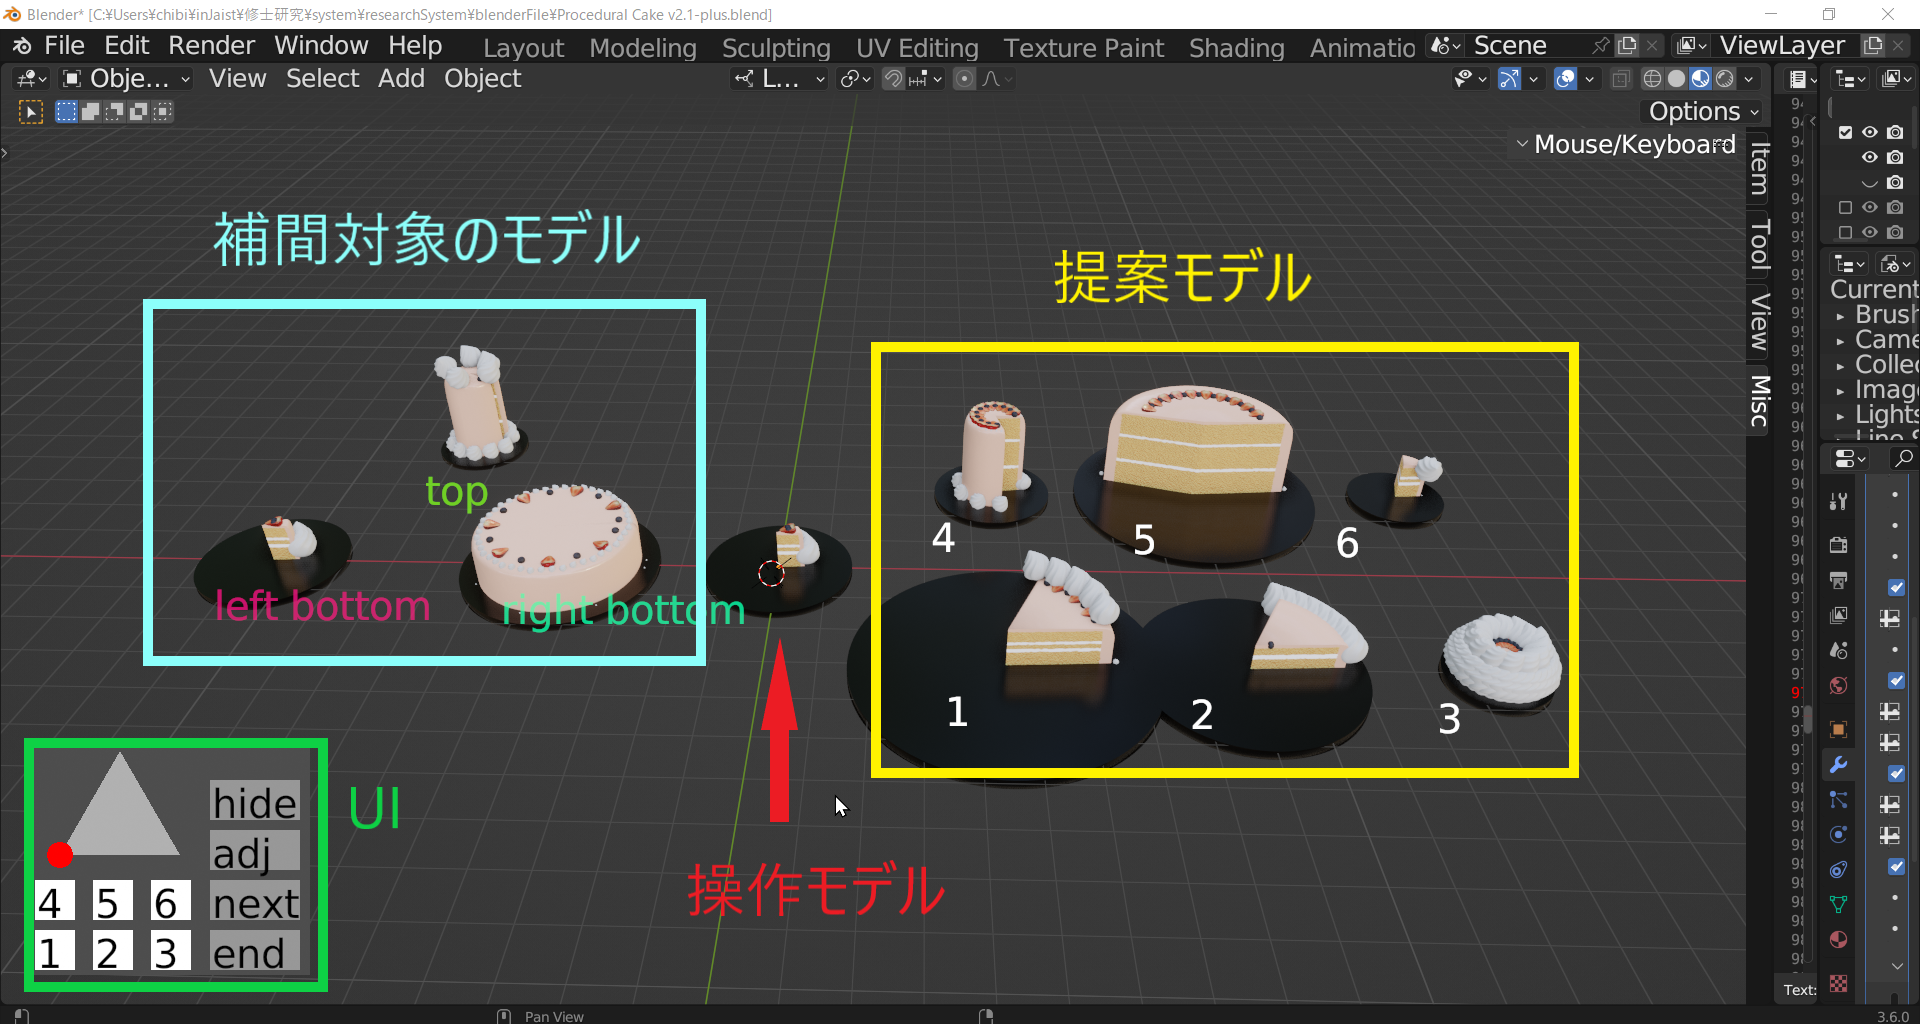
\includegraphics[scale=0.25]{./imgs/systemUse/init.png}
            \caption{システムの初期状態}\label{fig:systemOverViewInit}
	\end{center}
\end{figure}



\begin{figure}
  %\ContinuedFloat % 前の figure を継続
  \centering
  \begin{subfigure}{1\linewidth}
    \centering
    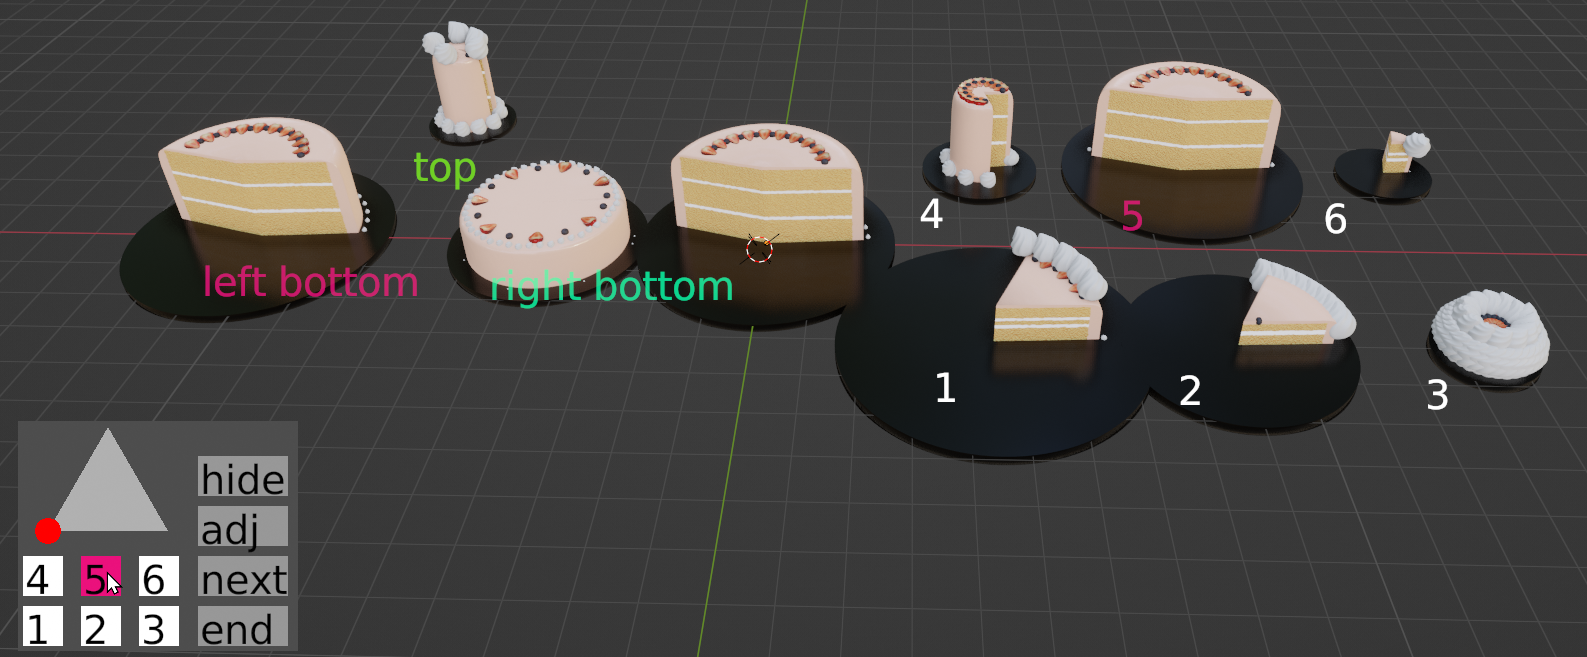
\includegraphics[scale=0.33]{./imgs/systemUse/select1.png}
    \caption{左下頂点に提案モデル5を選択}\label{fig:sOV_select1}
  \end{subfigure}\\
  \begin{subfigure}{1\linewidth}
    \centering
    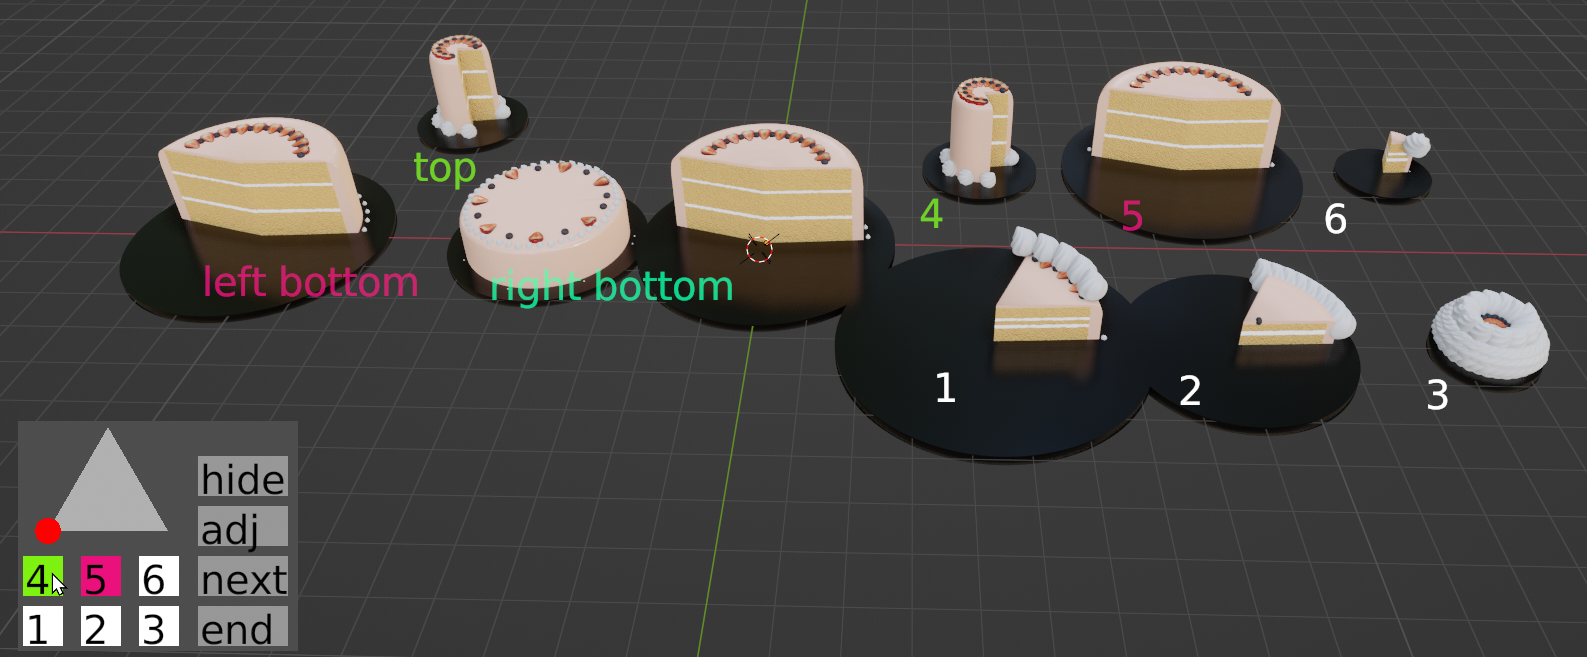
\includegraphics[scale=0.33]{./imgs/systemUse/select2.png}
    \caption{上頂点に提案モデル4を選択}\label{fig:sOV_select2}
  \end{subfigure}\\
  \begin{subfigure}{1\linewidth}
    \centering
    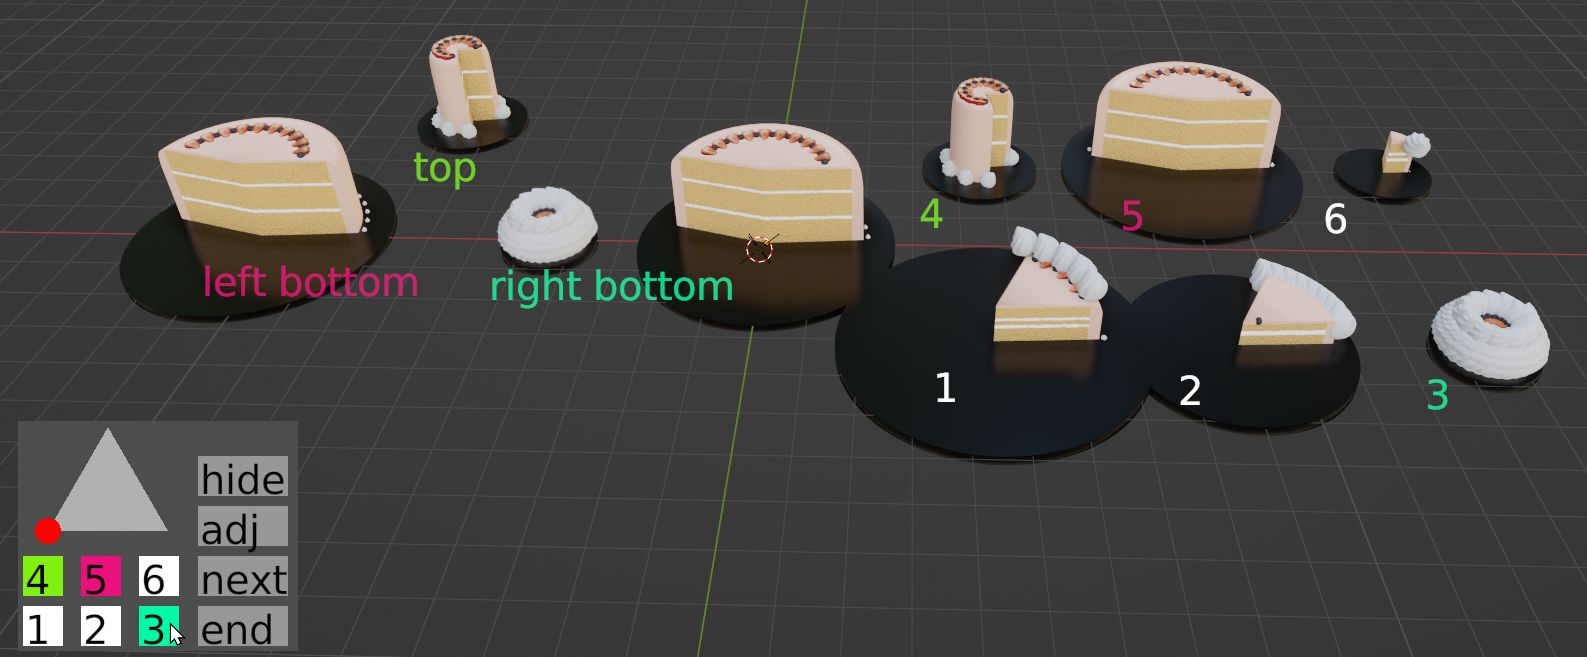
\includegraphics[scale=0.33]{./imgs/systemUse/select3.png}
    \caption{右下頂点に提案モデル3を選択}\label{fig:sOV_select3}
  \end{subfigure}\\
  \caption{実装システムの選択操作}\label{fig:systemOverViewSelect}
\end{figure}

\begin{figure}
  %\ContinuedFloat % 前の figure を継続
  \centering
  \begin{subfigure}{1\linewidth}
    \centering
    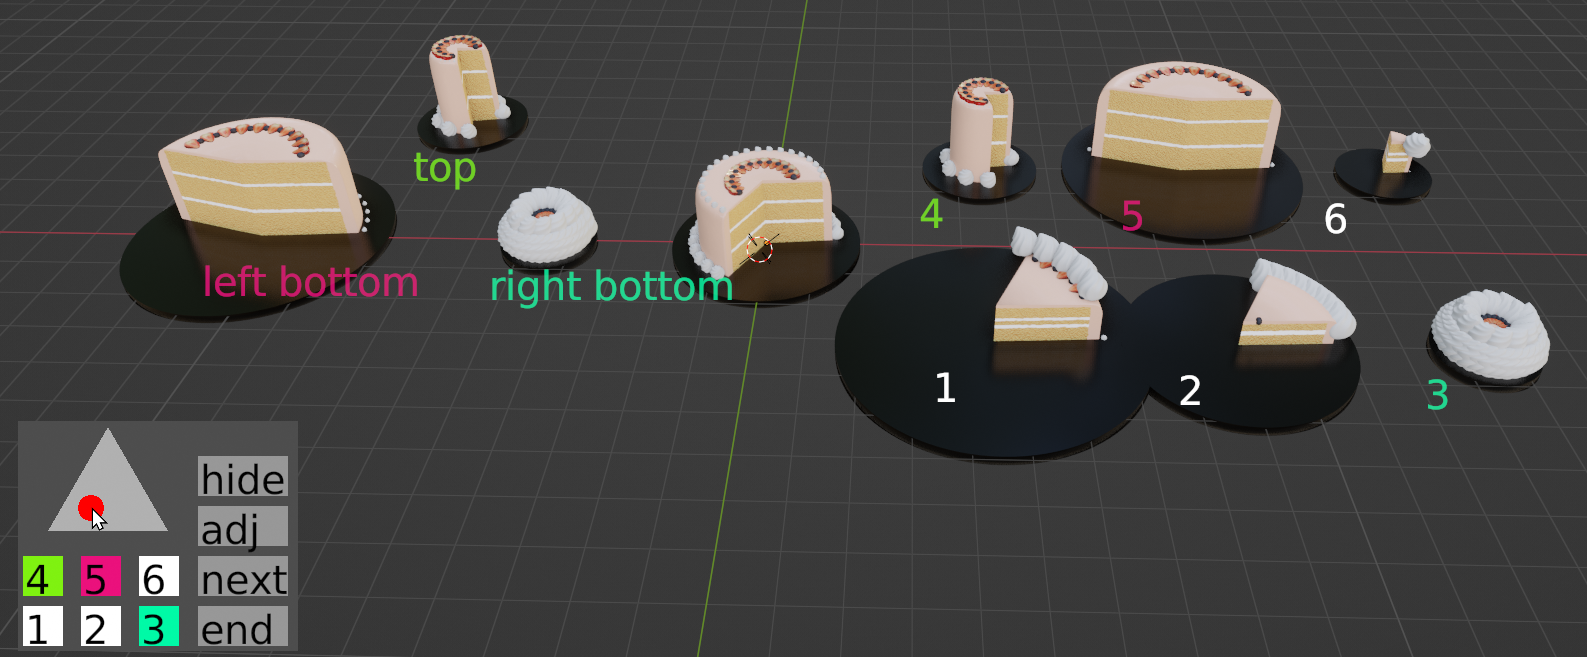
\includegraphics[scale=0.33]{./imgs/systemUse/inter1.png}
    \caption{補間操作($a=0.22,b=0.24$)}\label{fig:sOV_inter1}
  \end{subfigure}\\
  \begin{subfigure}{1\linewidth}
    \centering
    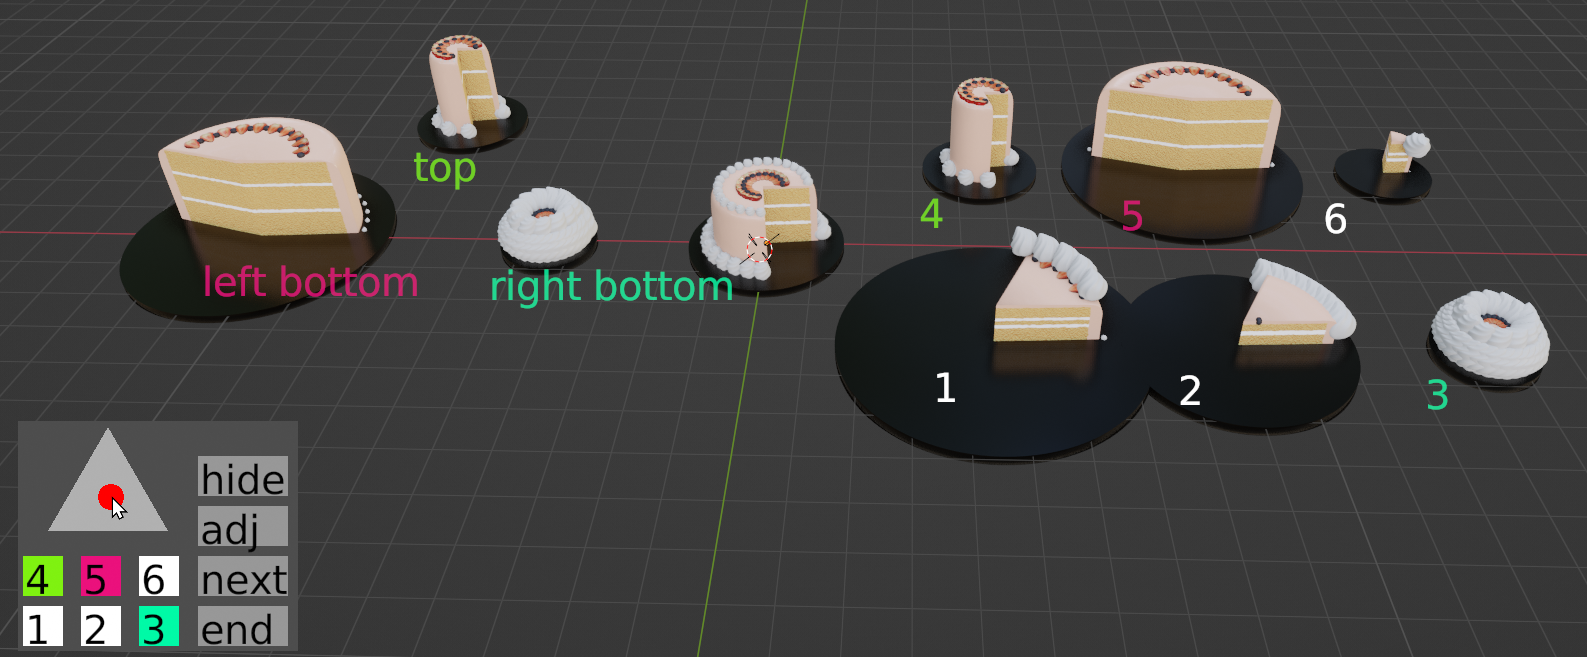
\includegraphics[scale=0.33]{./imgs/systemUse/inter2.png}
    \caption{補間操作($a=0.32,b=0.36$)}\label{fig:sOV_inter2}
  \end{subfigure}\\
  \begin{subfigure}{1\linewidth}
    \centering
    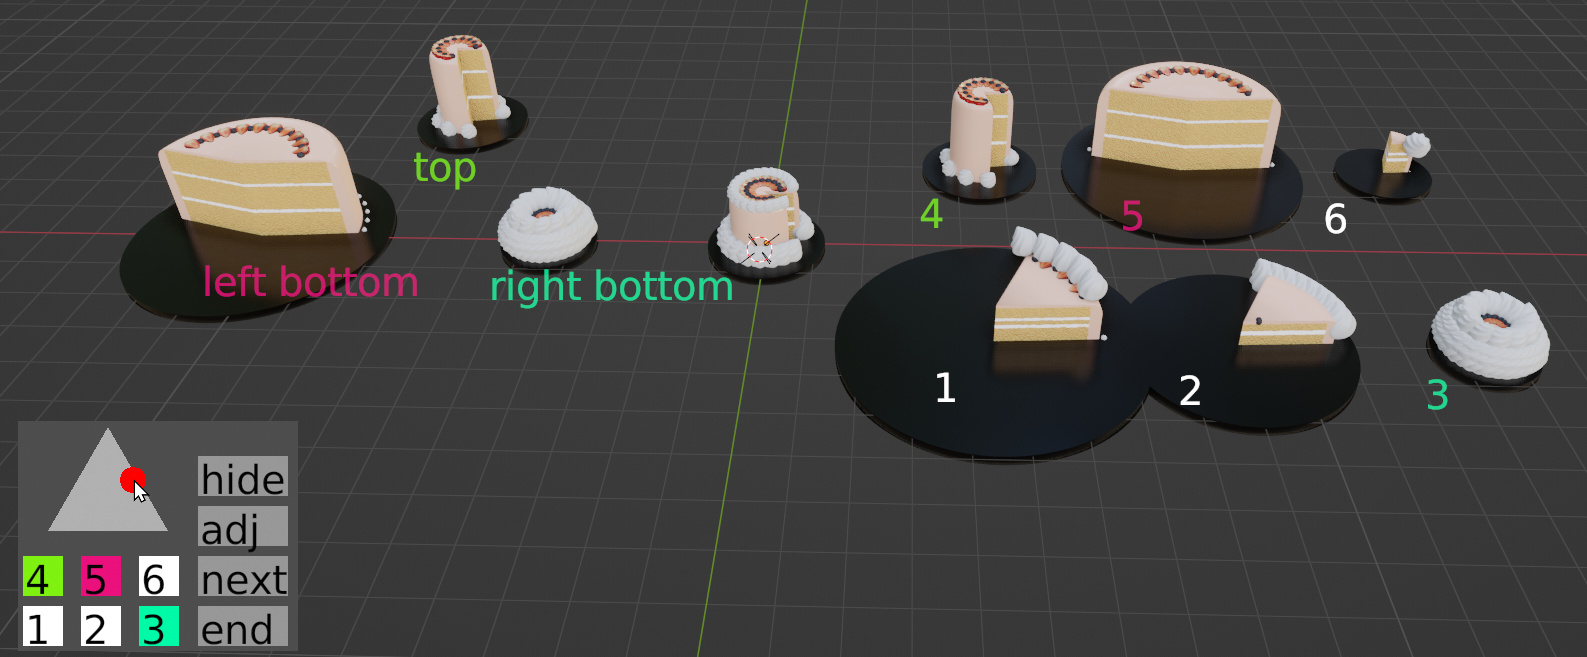
\includegraphics[scale=0.33]{./imgs/systemUse/inter3.png}
    \caption{補間操作終了($a=0.49,b=0.46$)}\label{fig:sOV_inter3}
  \end{subfigure}\\
  \caption{実装システムの補間操作}\label{fig:systemOverViewInter}
\end{figure}

\begin{figure}
  %\ContinuedFloat % 前の figure を継続
  \centering
  \begin{subfigure}{1\linewidth}
    \centering
    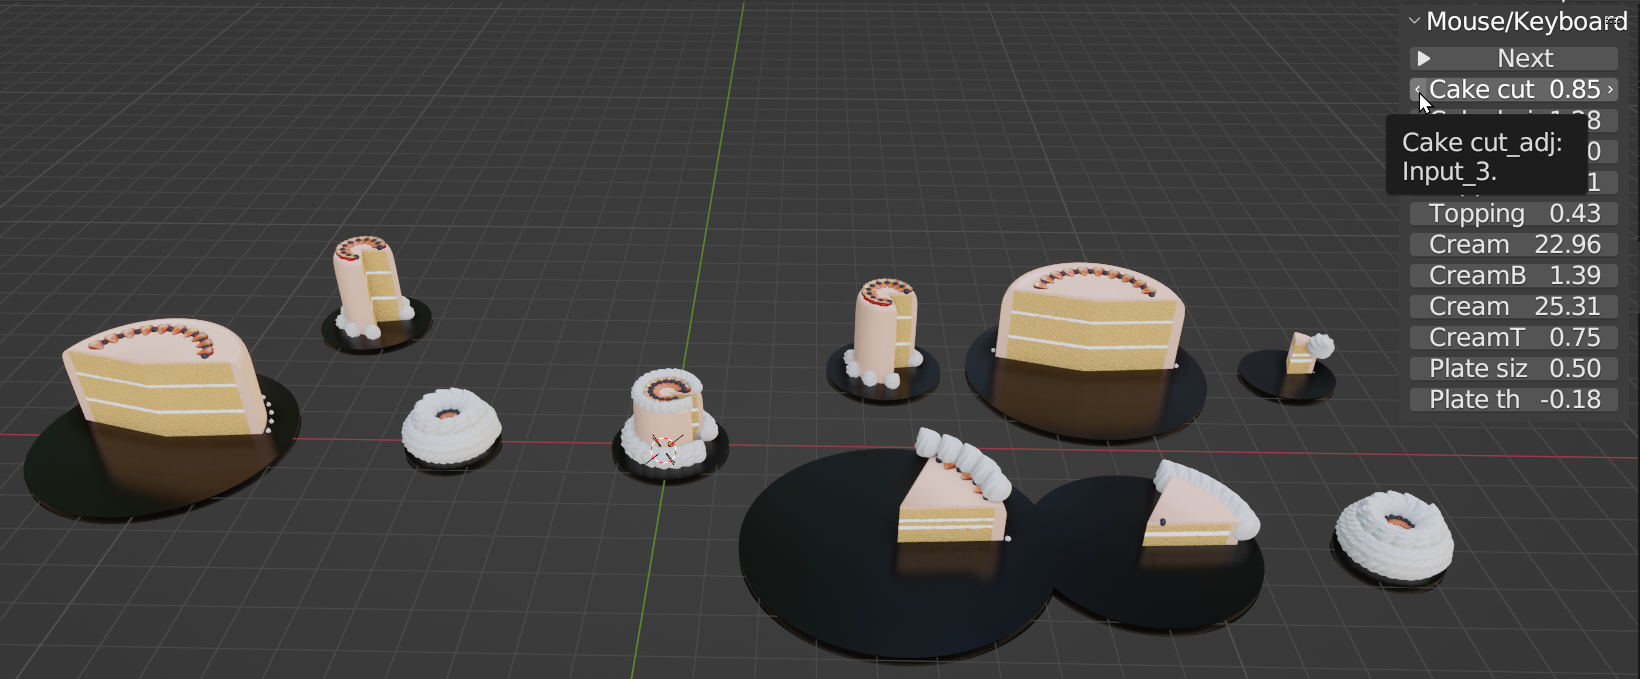
\includegraphics[scale=0.33]{./imgs/systemUse/adj0.png}
    \caption{微調整前(Cake cut = 0.85)}\label{fig:sOV_adj0}
  \end{subfigure}\\
  \begin{subfigure}{1\linewidth}
    \centering
    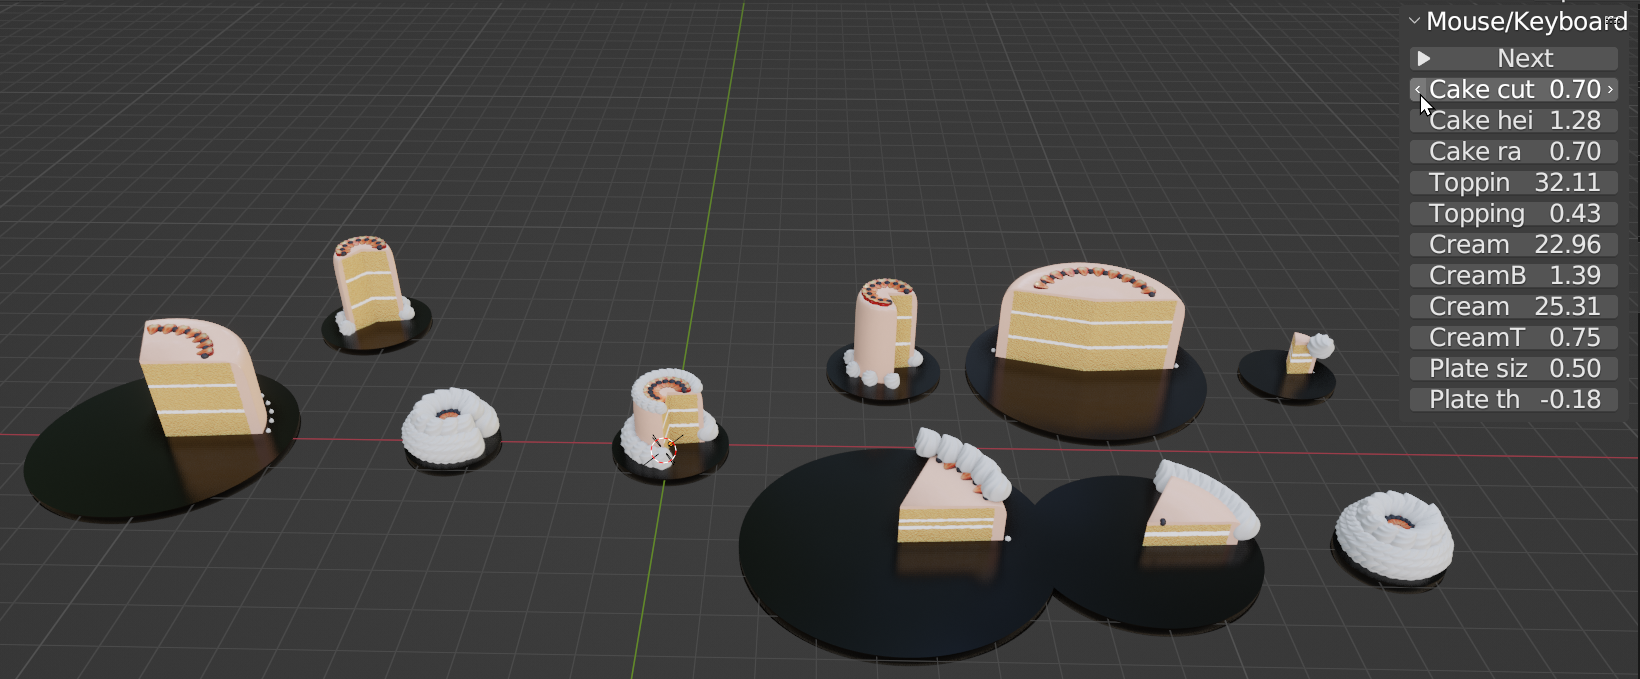
\includegraphics[scale=0.33]{./imgs/systemUse/adj1.png}
    \caption{微調整操作(Cake cut = 0.70)}\label{fig:sOV_adj1}
  \end{subfigure}\\
  \begin{subfigure}{1\linewidth}
    \centering
    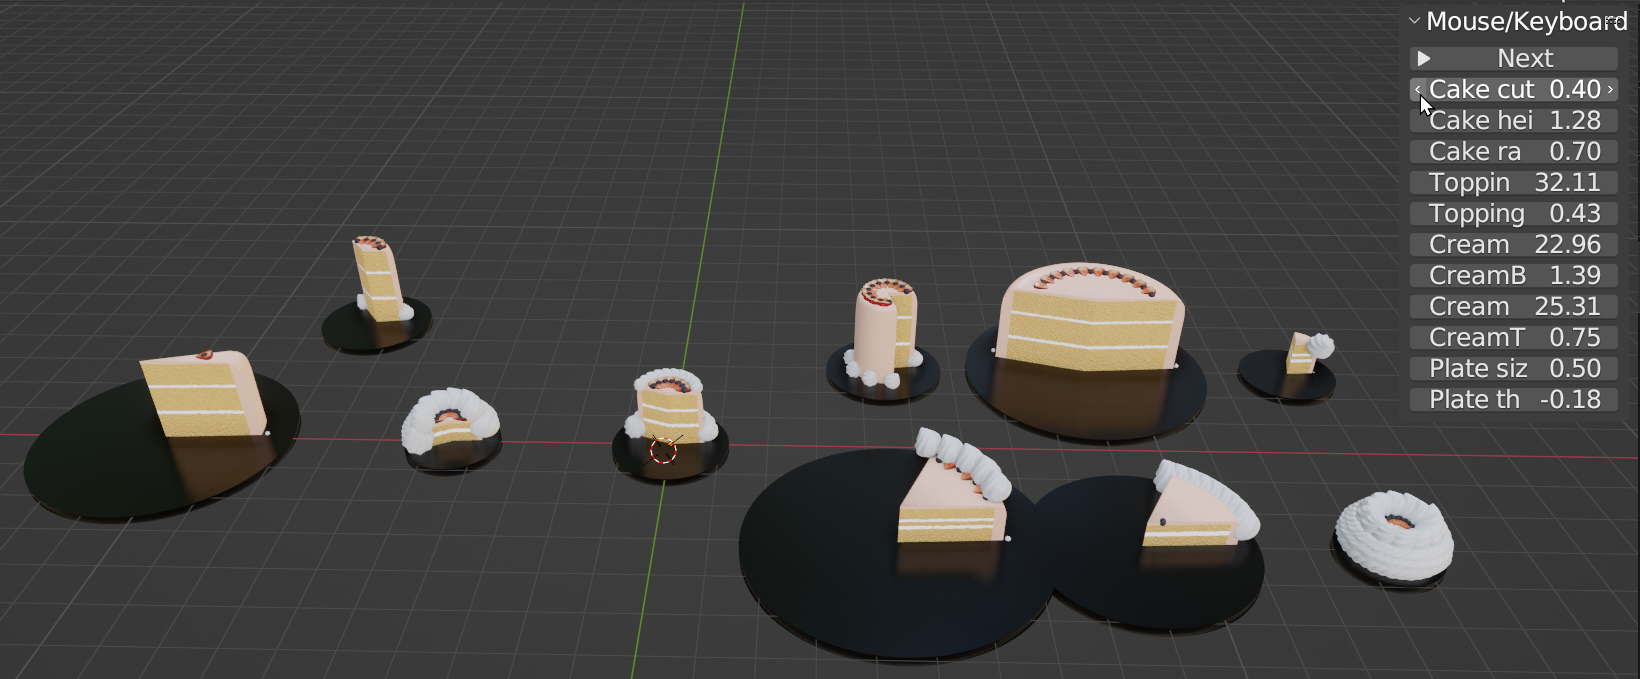
\includegraphics[scale=0.33]{./imgs/systemUse/adj3.png}
    \caption{微調整操作終了(Cake cut = 0.40)}\label{fig:sOV_adj2}
  \end{subfigure}\\
  \caption{実装システムの微調整操作}\label{fig:systemOverViewAdj}
\end{figure}
